\chapter{Metodología}
\label{sec::capitulo3}

\section{Detección de somnolencia}
\subsection{Detección de rostro}
El primer paso para poder realizar cualquier análisis en nuestras imágenes es detectar el rostro del conductor, para poder así calcular las métricas deseadas en base a la detección correcta de un rostro en la imagen. La detección consiste de dos partes diferentes, ambas necesarias para poder calcular correctamente lo que se busca. El primer paso es detectar solamente la presencia de un rostro. Existen algoritmos capaces de lograr esto los cuales están documentados como opciones funcionales. Para este objetivo, se utiliza el HOG que forma parte de la librería Dlib, el cual es algoritmo ya entrenado específicamente para la detección de rostros (\cite{MinhasPERCLOS}).

Tras la detección del rostro, es necesario utilizar un detector de puntos faciales, que también forma parte de la librería Dlib. Lo que este algoritmo logra es una vez con el rostro detectado, localiza 68 puntos a lo largo del rostro, ofreciendo un mapeo del rostro que permite calcular métricas relacionadas a distancias en distintas partes del rostro. La Figura \ref{fig:68} muestra como se mapean los 68 puntos a lo largo del rostro. Se puede apreciar que se genera un contorno del rostro, los ojos, la nariz, y la boca. 

\begin{figure}[h!]
    \centering
    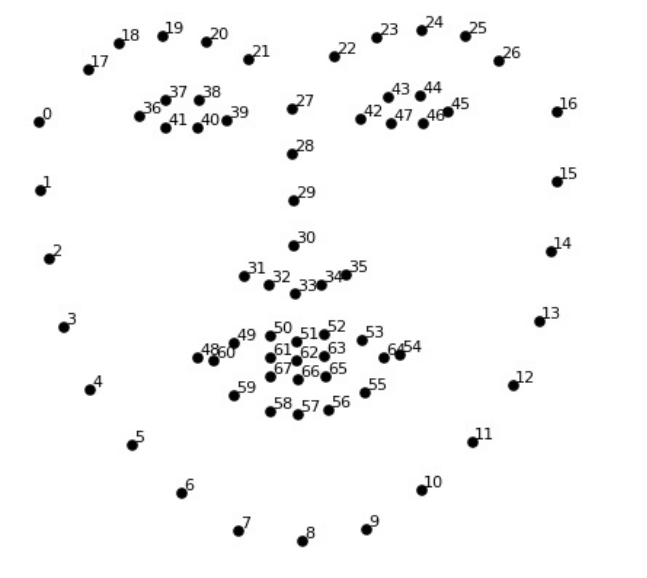
\includegraphics[width=0.5\linewidth]{figures/68points.png}
    \caption{Mapeo del rostro con 68 puntos(\cite{MinhasPERCLOS})}
    \label{fig:68}
\end{figure}

Es a través de los puntos que forman los ojos y la boca que se pueden realizar los cálculos matemáticos para determinar si el conductor se encuentra en estado de somnolencia o no, por lo que una vez establecidos los 68 puntos, podemos continuar con el cálculo de las métricas PERCLOS, duración de parpadeo, detección de bostezo y orientación de la cabeza. 

\subsection{Cálculo de PERCLOS y duración de parpadeo}
Para ser capaces de calcular el PERCLOS, es necesario calcular primero el EAR. El EAR se obtiene a través de una fórmula que utiliza los 6 puntos del ojo obtenidos con el detector de Dlib. Realizando restas, sumas, y divisiones entre estos 6 puntos, el algoritmo es capaz de determinar que tan abierto o que tan cerrado se encuentra el ojo, siempre y cuando se tengan estos 6 puntos, que funcionan como esquinas del ojo que se acercan o alejan entre sí dependiendo de la apertura del ojo. 
\[
\mathrm{EAR} = \frac{|\mathrm{P}_2 - \mathrm{P}_6| + |\mathrm{P}_3 - \mathrm{P}_5|}{2|\mathrm{P}_1 - \mathrm{P}_4|}
\]

El EAR de ojo abierto y cerrado son medidas que pueden variar de persona en persona, y para poder hacer que esta variabilidad no fuera un factor que pueda afectar nuestro proyecto, se aplicó una fase de calibración al programa. Dentro de esta fase de calibración se pide que el usuario mantenga los ojos abiertos como lo haría de forma regular durante un tiempo determinado, tras el cual se les pide que mantengan los ojos cerrados de forma regular por la misma cantidad de tiempo. Dentro de estos tiempos mencionados anteriormente, se van obteniendo los valores de EAR fotograma por fotograma de cada uno de los dos estados, tras lo cual se promedian sus valores, y a partir de estos se determina el valor de EAR de ojo abierto y cerrado del usuario.

El PERCLOS está establecido como la medición de cuanto tiempo el ojo estuvo por lo menos 80\% cerrado durante un periodo de tiempo determinado. Esto significa que podemos establecer que cuando nuestro EAR tenga un valor de 0.2 o menor, el ojo se encuentra cerrado (\cite{MinhasPERCLOS}). 

Finalmente, la ventana de tiempo que se eligió para el cálculo del PERCLOS es de 30 segundos, esto buscando tener una ventana de tiempo que sea pequeña para un monitoreo constante, pero que mantenga un comportamiento de resultados parecido a ventanas de tiempo usualmente utilizadas, como 1 minuto. Para nuestra implementación se utilizó una ventana de tiempo móvil, esta recopila toda la información obtenida durante estos 30 segundos, pero permitiendo que se refresque con cada segundo que pasa. Dentro de esta ventana de tiempo móvil se obtiene el valor de EAR en cada fotograma y se promedia para obtener un porcentaje representativo de la cantidad de tiempo que un ojo ha permanecido por debajo del 20\% de apertura durante los últimos 30 segundos. Para el contexto de nuestro detector de somnolencia, se decidió que se utilizaría el porcentaje de 15\% como umbral para determinar si el usuario está sufriendo algún episodio de somnolencia (\cite{LibroPERCLOS}).

Para el cálculo de la duración de un parpadeo, se utiliza también el EAR obtenido con la ayuda de Dlib, pero se sigue un procedimiento diferente para establecer el valor. Dentro de la literatura existen múltiples formas de determinar un parpadeo, algunas lo consideran desde el momento en que empieza a cerrarse el ojo hasta el momento en el que se vuelve a abrir, y otras lo consideran únicamente el tiempo que permanece cerrado. Para el contexto de nuestro proyecto, definimos el parpadeo únicamente como el tiempo que el ojo permanece totalmente cerrado. Ahora, para poder determinar cuando sucede un parpadeo, se utilizó el mismo umbral del 20\% de apertura utilizado en el cálculo del PERCLOS, pues es lo suficientemente permisivo al detectar parpadeos para que los detecte de forma consistente sin equivocarse de forma excesiva. Finalmente, para poder determinar cuanto tiempo permanece cerrado el ojo, al momento que se cruce el umbral del 20\% de apertura del ojo, se activa un contador, el cual deja de contar al momento que se determine que el ojo supere este umbral. A su vez, mientras el EAR se mantenga por debajo de un segundo umbral dictado por el 70\% de apertura, se le permite reanudar el contador, permitiendo que picos pequeños que pueden suceder al tener el ojo cerrado puedan ser ignorados para continuar el conteo del parpadeo sin interrupciones de poca relevancia. Para este proyecto, nos basamos en artículos científicos publicados en el pasado para que el detector de somnolencia determinara que cualquier parpadeo superior a 500 milisegundos sea indicativo de episodios de fatiga, lo cual permite que se dispare una alarma (\cite{BlinkDuration}).

Parte importante de nuestro detector de PERCLOS y duración de parpadeo es un filtro adaptativo implementado para poder adaptarse a como va evolucionando el EAR del usuario con el tiempo. Este filtro adaptativo obtiene los valores del EAR del usuario y los aplica en filtro de mediana con una ventana móvil, siendo esta de longitud de 5, lo cual significa que obtiene los valores de los últimos 5 fotogramas incluyendo el actual y obtiene la mediana de estos para determinar un valor. Tras esto se le aplica un segundo filtro de media móvil, pero este con una ventana móvil de longitud de 30, obteniendo los últimos 30 fotogramas que fueron pasados por el filtro de mediana y obteniendo un único valor para el fotograma actual al obtener su promedio. Aplicar estos dos filtros nos permite tener un umbral adaptativo que pueda cambiar a partir del comportamiento del EAR del usuario de forma consistente, pues su combinación elimina los picos que se puedan encontrar al momento de cerrar el ojo al igual que suavizar la curva de la gráfica para no tener cambios de valores bruscos. En nuestro programa, al momento en el que el PERCLOS supere un porcentaje del 15 porciento se encenderá una alarma para el conductor, este porcentaje lo elegimos basándonos en artículos científicos anteriores (\cite{MinhasPERCLOS}).

Buscando determinar si nuestro algoritmo detecta parpadeos de la forma deseada, se evaluó en el conjunto de datos EyeBlink8, que cuenta con imágenes de 8 sujetos grabados en interiores. Cuenta con anotaciones por fotograma de cuando el sujeto parpadea. El conjunto de datos cuenta con 387 eventos de parpadeo distintos, repartidos de forma aleatoria entre los 8 sujetos. Los parpadeos del conjunto de datos están registrados en distintos archivos TAG, que tienen los datos del rostro anotados de fotograma a fotograma, detallando los momentos en los que el ojo del sujeto se mantiene cerrado y cuál número de evento de parpadeo es el actual junto con el número del fotograma en el que sucede cada cosa. En la figura \ref{fig:eb8} se encuentra una muestra tomada de uno de los videos disponibles en el conjunto de datos de EyeBlink8.

\begin{figure}[h!]
    \centering
    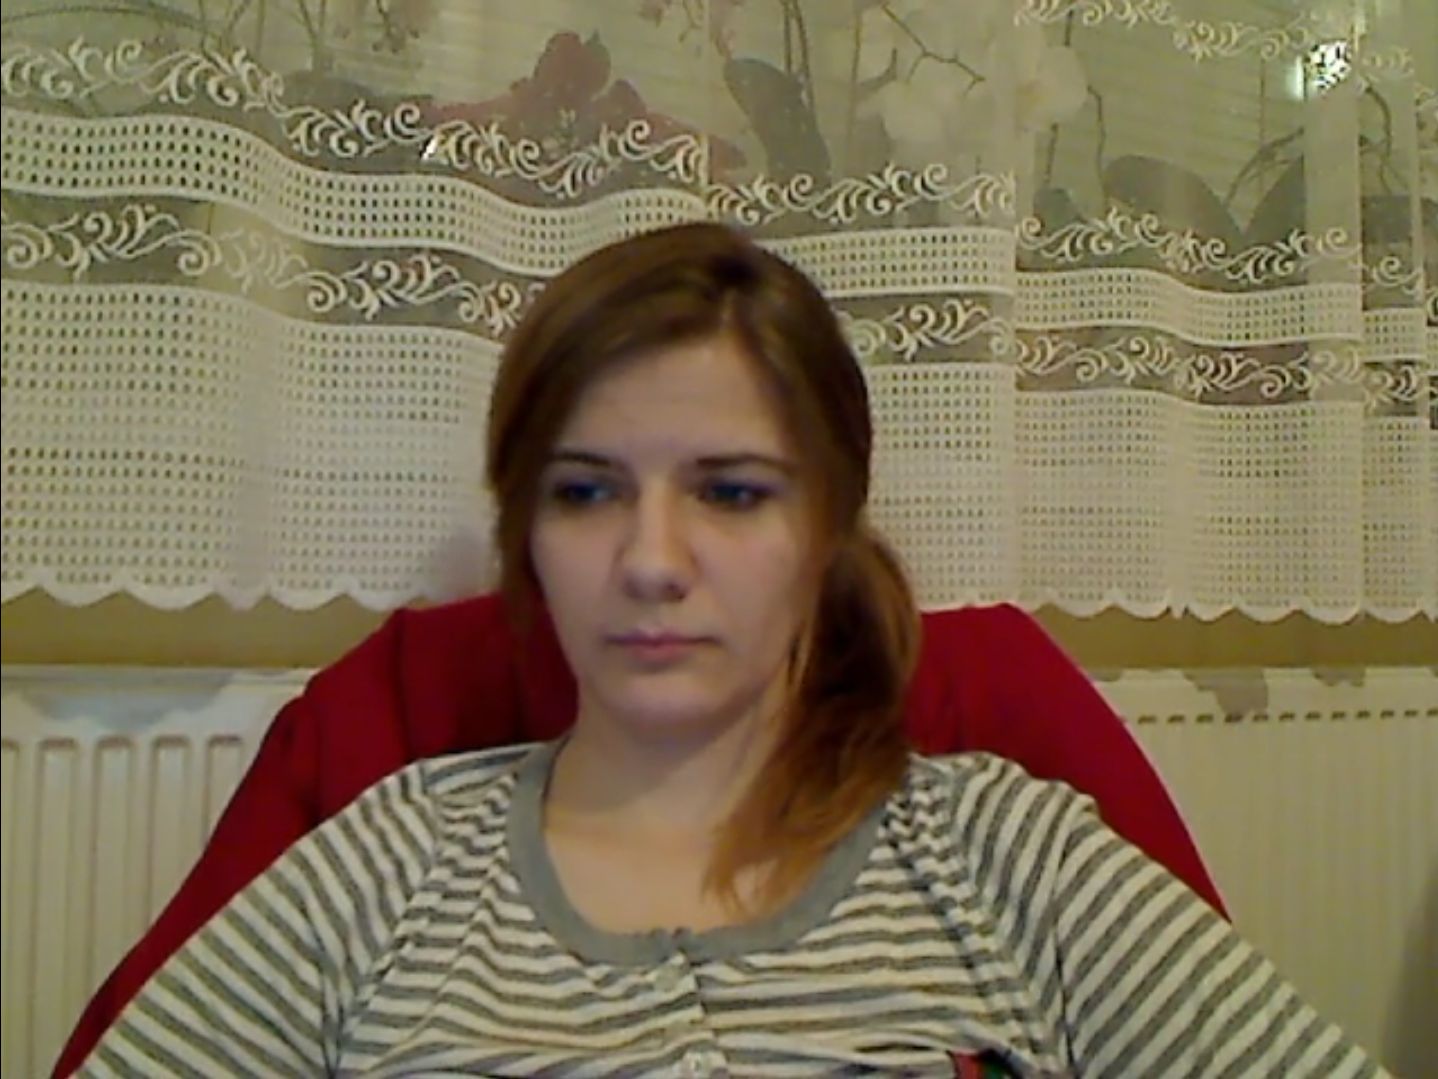
\includegraphics[width=0.5\linewidth]{figures/muestra eb8.png}
    \caption{Imagen de muestra del conjunto de datos de EyeBlink8}
    \label{fig:eb8}
\end{figure}

Aparte de la evaluación realizada con el conjunto de datos de EyeBlink8 se realizó otra con el conjunto de datos DMD, el cual cuenta con una mayor variación de sujetos en sus grabaciones, utilizando las anotaciones de \textit{open}, \textit{opening}, \textit{close} y \textit{closing}. Este segundo conjunto de datos está separado en imágenes, cada una siendo un fotograma de uno de los videos incluidos en este, estas imágenes están nombradas a partir del video al que pertenecen y la parte del video en la que se encuentran, aparte de esto, las imágenes están separadas por carpetas, las cuales están nombradas a partir del tipo de anotación al que pertenecen las imágenes que contienen, permitiendo la distinción de los eventos de parpadeos para nuestra evaluación. En las figuras \ref{fig:close} \ref{fig:open} se encuentran muestras de dos de los tipos de anotaciones que se pueden encontrar en el conjunto de datos del DMD.

\begin{figure}[h!]
    \centering
    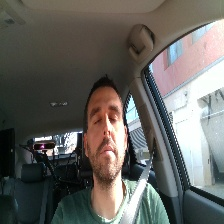
\includegraphics[height=0.30\textheight,keepaspectratio]{figures/muestra close.jpg}
    \caption{DMD: Hombre caucásico con los ojos cerrados (\cite{DMD})}
    \label{fig:close}
\end{figure}

\begin{figure}[h!]
    \centering
    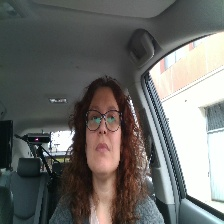
\includegraphics[height=0.30\textheight,keepaspectratio]{figures/muestra open.jpg}
    \caption{DMD: Mujer caucásica con lentes con los ojos abiertos (\cite{DMD})}
    \label{fig:open}
\end{figure}

Finalmente, se entrenó una red neuronal convolucional para detección de parpadeo para ambos conjuntos de datos, buscando tener un punto de comparativa para el algoritmo propuesto y determinar si este es realmente competitivo al ponerlo en contra de otros métodos de detección para estas dos bases de datos específicamente. La CNN fue entrenada a partir del conjunto de datos del EyeBlink8, pues se tiene una clara distinción de cuando se tiene cerrado o no el ojo. Para el uso del conjunto de datos en el entrenamiento de la CNN, se realizaron recortes de los rostros de los sujetos utilizando el detector de rostros HOG de Dlib, al igual que un redimensionamiento de las imágenes a 112$\times$112 en cada fotograma de cada video como formas de preprocesamiento para el entrenamiento correcto de la CNN. La CNN cuenta con cuatro bloques convolucionales, cada uno compuesto por una capa de convolución, seguida por una capa de dropout, seguida por una capa de activación de LealyReLU, finalizada por una capa de batch normalization. Tras los bloques convolucionales se tienen una capa de global average pooling, tras la cual se tienen dos bloques de capas densas, que contienen una capa densa, una capa de activación de LeakyReLU, seguida por una capa de batch normalization, y para el caso del segundo bloque, se finaliza con una capa de sigmoide para poder extraer la respuesta decidida por la red neuronal. 

La arquitectura utilizada en la red neuronal de detección de parpadeos fue elegida debido a que se tiene planeado utilizar una estructura más robusta y exigente para la red neuronal que se utiliza para la detección de distracción, y por eso, en dado caso se fuera a implementar esta CNN, debe de ser ligera para su funcionamiento correcto dentro de la raspberry pi en la que se va a correr el programa.

Con el fin de determinar la funcionalidad de la CNN entrenada se le aplicó una prueba de forma similar a la del PERCLOS, utilizando el conjunto de datos de somnolencia del DMD para su evaluación. A diferencia de la prueba anterior, para el uso de este conjunto de datos se requirió cierto preprocesamiento a las imágenes que lo componen, para esto, primero se realizó un preprocesamiento de las imágenes del conjunto de datos de forma similar al que se realizó para el conjunto de datos del EyeBlink8 para poder alimentarlas a la CNN y poder alivianar su carga de procesamiento.

\subsection{Detección de bostezo}
La detección de bostezo tiene un procedimiento similar al del cálculo del PERCLOS, con la única diferencia se utiliza el MAR en vez de EAR. En la formula utilizada se cuenta con los 8 puntos que generan el contorno de la boca. E igualmente que con los ojos, usando estos 8 puntos como esquinas se puede determinar que tan abierta o cerrada se encuentra la boca, y una vez establecido si esta abierta o no la boca, determinar si el conductor se encuentra bostezando o no. 
\[
\mathrm{MAR} = \frac{|\mathrm{P}_2 - \mathrm{P}_9| + |\mathrm{P}_3 - \mathrm{P}_7| + |\mathrm{P}_4 - \mathrm{P}_6|}{3|\mathrm{P}_1 - \mathrm{P}_5|}
\]

% Esto pudiera mejorarse, porque parecer ser que en realidad los bostezos *promedio* son los que duran entre 4-6 segundos, pero como el equipo lo discutió en su momento, hay bostezos que duran como 2 segundos. Y es que creo que hay artículos que encuentran que, si bien la duración de bostezos varía mucho entre sujetos (unos bostezando, en general, por más tiempo que otros), la duración entre bostezos es consistente para un mismo sujeto. Además, puede ser que esos 4-6 segundos estén considerando todo el ciclo del bostezo: cuando alguien empieza a abrir la boca, cuando está en su peak, y cuando la está cerrando, pero el MAR de 0.5 tiene la limitante de que es más representativo de la boca estándo más cerca de su peak que de la boca abriendose o cerrándose apenas. Mi punto es: teníamos razones para esperarnos 4 segundos de predicciones pseudo-consecutivas para declarar un episodio de bostezo, pero también teníamos razones para probar diferentes tiempos y ver qué resultados teníamos. Solo habría que ver como condensar esta redacción, y respaldarla con referencia(s).  
Basándonos en el estado del arte, se establece en el algoritmo que el valor de MAR para encontrar un bostezo es de 0.5 (\cite{Bostezo}). Para la implementación en tiempo real, primero establecimos que se haría una detección de bostezo cuando este valor de MAR se encontrara de manera consecutiva durante 4 segundos, de acuerdo a lo encontrado en el estado del arte (\cite{Bostezo}). Sin embargo, pruebas iniciales detectando bostezos con el MAR nos mostraron que había momentos donde Dlib no detectaba un rostro, y cuando eso pasaba, ya no se cumplía el criterio de detección consecutiva, y por tanto se reiniciba el conteo de los 4 segundos. Por lo tanto acordamos que, tras capturar una imagen de la cámara, tanto si no se detectaba un rostro, como si tras detectarlo el MAR bajaba del threshold, no volveríamos a empezar otros 4 segundos, sino que el conteo de tiempo acumulado de bostezo disminuiría con cada ciclo.

Para el análisis de la detección de bostezo en nuestro algoritmo, se recurre al conjunto de datos de \textbf{YawDD} (\cite{YawDD}). Incluye 349\footnote{En el sitio web original se menciona que son 351 videos en total, pero al descargar el conjunto de datos contamos únicamente con 349 de ellos.} videos, grabados dentro de un carro real con una resolución de 640$\times$480 a 30 FPS, y con diferentes conductores: hombres y mujeres, con o sin lentes, y de diferentes grupos étnicos. Los videos contienen episodios donde los conductores están: 1) en conducción normal (sin hablar), 2) hablando y/o cantando, y 3) bostezando; lo hacen en diferentes condiciones de iluminación. Hay dos conjuntos principales de videos: grabados desde el espejo retrovisor (320 videos), y grabados desde el tablero del carro (29 videos). Por estas razones las imágenes tienen nombres como \verb|"1-FemaleNoGlasses-Yawning.avi"|, dentro de carpetas que indican la ubicación de la cámara, y que indican si son hombres o mujeres. Ejemplos de imágenes de los 3 grupos de actividades que realizan los conductores se encuentran en las Figuras \ref{fig:YawDD_p34}, \ref{fig:YawDD_p38}, y \ref{fig:YawDD_p41}.

\begin{figure}[h!]
    \centering
    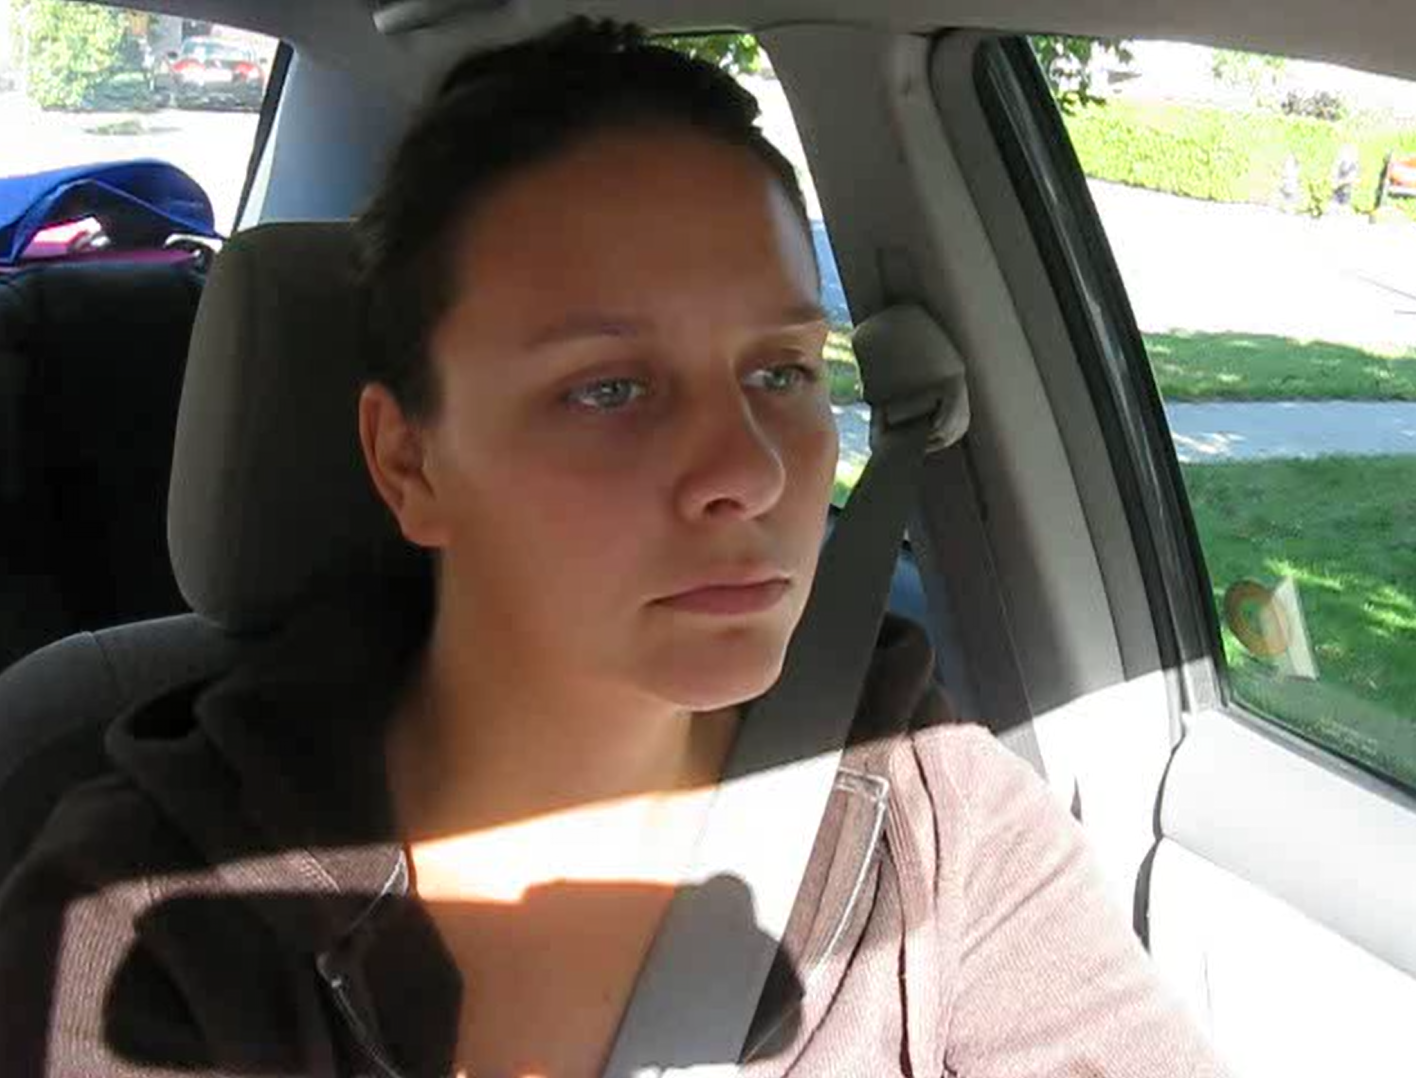
\includegraphics[width=0.5\linewidth]{figures/yawdd_participant_34_female_normal.png}
    \caption{YawDD: Mujer caucásica en conducción normal. (\cite{YawDD})}
    \label{fig:YawDD_p34}
\end{figure}

\begin{figure}[h!]
    \centering
    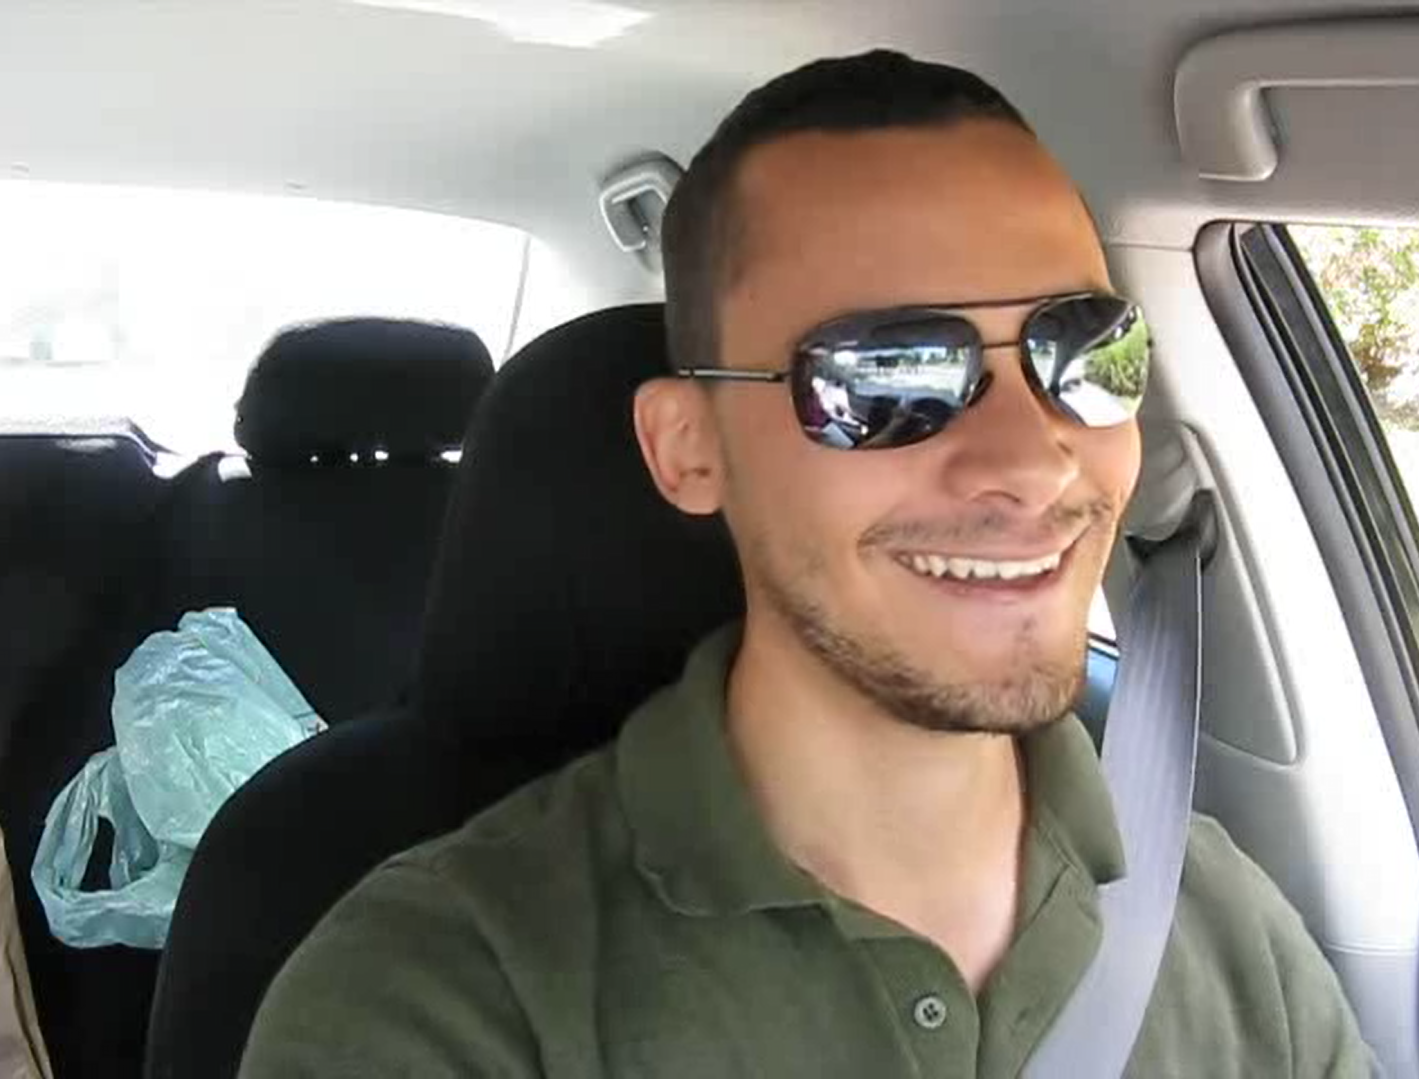
\includegraphics[width=0.5\linewidth]{figures/yawdd_participant_38_male_talking.png}
    \caption{YawDD: Hombre africano hablando. (\cite{YawDD})}
    \label{fig:YawDD_p38}
\end{figure}

\begin{figure}[h!]
    \centering
    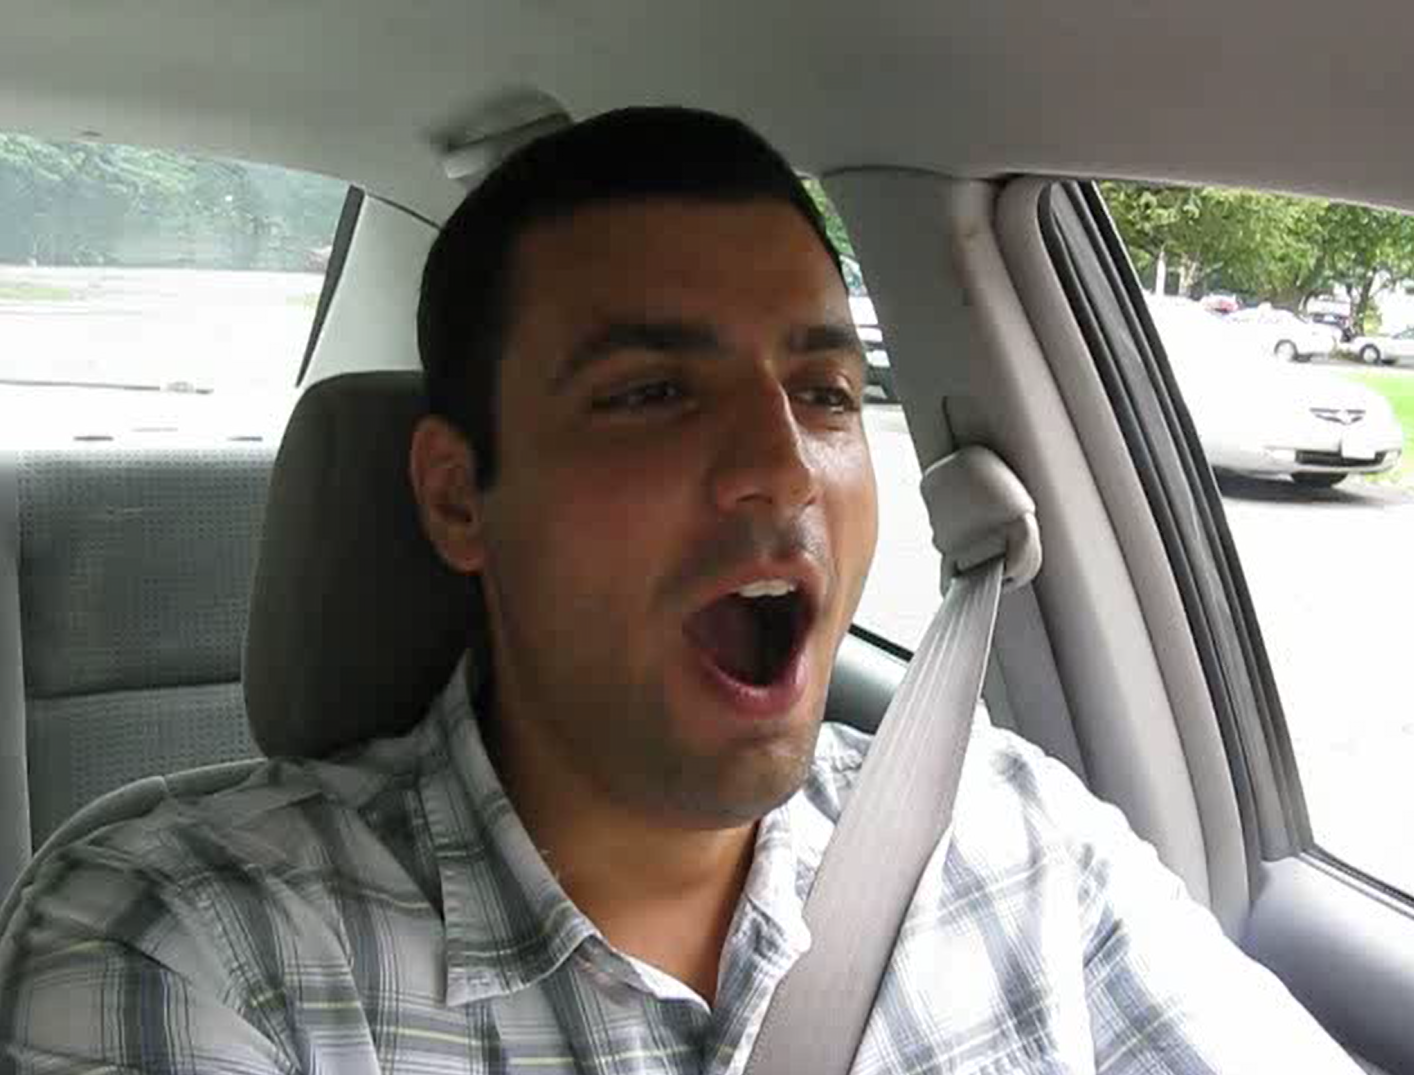
\includegraphics[width=0.5\linewidth]{figures/yawdd_participant_41_male_yawning.png}
    \caption{YawDD: Hombre del medio oriente bostezando. (\cite{YawDD})}
    \label{fig:YawDD_p41}
\end{figure}

Este conjunto de datos tiene una peculiaridad: a pesar de que tiene videos cuyos  nombres mencionan una actividad general que realiza el conductor en cuestión, no contiene anotaciones a nivel imagen que nos permita validar que las predicciones de nuestro algoritmo sean correctas. Tras investigar, nos encontramos con \textbf{YawDD+} (\cite{YawDDPlus}), un conjunto de anotaciones para cada imagen de cada video de YawDD. Ellos desarrollaron una \textit{pipeline} semi-automatizada con verificación humana para hacer las anotaciones, alcanzando una exactitud de 99.34\%. Las anotaciones son archivos .txt de una sola línea cuyo contenido es de la forma \verb|"[anotación] [coordenadas_normalizadas]|". Las anotaciones son \verb|0| ("normal") o \verb|1| ("bostezo") y las coordenadas normalizadas marcan los extremos de recuadros utilizados para aplicaciones de detección de objetos. Los videos donde alguien bosteza no se componen enteramente del episodio de bostezo. Es decir, dentro de un video, puede haber imágenes donde se etiqueta como \verb|0|, y en algún punto del video haber uno o más episodios de bostezo, anotados con \verb|1|. Cada video tiene una carpeta correspondiente que cuenta con $n$ archivos .txt, uno por cada imagen del video. YawDD+ contiene 349 carpetas de anotaciones, cantidad que corresponde a los 349 videos que tenemos de YawDD. Fue así que pudimos trabajar con YawDD como se esperaba. 

Sin embargo, como este conjunto de datos se creó para detección de objetos, hay un total de 287,225 anotaciones en archivos .txt. Tras iniciar una operación de copiado y pegado de la carpeta con las anotaciones a otro directorio, y ver el tiempo que tardaba en realizarla, se consideró que esta estructura haría también que cualquier evaluación del algoritmo de detección de bostezo que hiciéramos se tardaría mucho por la lectura de archivos. Por tanto, se creó con un LLM un script de Python que, para cada video, concatenara todas las anotaciones en un solo .txt dentro de carpetas de Dash y Mirror, como el conjunto de datos original, y a partir de esos archivos poblar un JSON con información de conteo de imágenes, conteo de imágenes de bostezo, y las anotaciones de bostezo / no bostezo para cada video. También se generó otro script para tener 2 JSONs en los cuales vivieran dos subconjuntos "virtuales" (en lugar de almacenar dos veces el conjunto de datos en directorios diferentes, tener JSONs cuyos objetos tengan atributos que apunten a los videos deseados) de datos. Uno con el cual evaluar el algoritmo de detección de bostezo, y modificar la duración de segundos requeridos para detectar bostezos dependiendo de los resultados obtenidos en caso de verlo útil, y el otro para validarlo con videos de los cuales no hayamos obtenido retroalimentación previa.

% aquí estaría cool mostrar una imagen de los clips que se generaban
Tras empezar a probar el algoritmo con el conjunto de datos de experimentación, notábamos que tenía una precisión alta, pero una exhaustividad muy baja: habían muchos bostezos verdaderos que \textit{no} se estaban detectando. Para averiguar por qué ocurría esto, generamos un script de Python que extrajera clips de videos cuyas anotaciones indicaban episodios de sueño, y que además anotara esos videos con información acerca del MAR, la detección facial, y demás información que nos pudiera ser útil para encontrar posibles errores. No fue necesario revisar muchos clips para darnos cuenta que el problema era que en ciertas orientaciones de la cabeza, Dlib simplemente no era capaz de detectar un rostro. Probamos con diferentes thresholds para el MAR y duraciones mínimas de bostezo detectado para catalogar un episodio de bostezo, pero los resultados fueron similares. Por ello, decidimos experimentar con un enfoque un poco más demandante computacionalmente, pero que la literatura nos muestra que entrega mejores resultados: una CNN. 

\subsubsection{Entrenamiento}

Considerando que la velocidad de inferencia de la CNN necesitaba ser alta, se comenzó entrenando modelos con imágenes de entrada de $224\times224$. No obstante, al evaluar el costo computacional con los recursos disponibles, se optó por reducir la resolución a $112\times112$, obteniendo resultados equivalentes con un tiempo de entrenamiento e inferencia significativamente menor. Tras realizar diversas pruebas de ajuste en la cantidad de capas convolucionales, funciones de activación, capas densas y regularización, se consolidó la arquitectura presentada en la Tabla \ref{tab:tabla CNN yawning}.

La red está compuesta por 4 bloques convolucionales secuenciales y un bloque de capas densamente conectadas. Cada bloque convolucional sigue la misma estructura base de cinco etapas:
\begin{enumerate}[noitemsep,topsep=0pt]
    \item \textbf{Convolución 2D}: Filtros de $3\times3$ con \textit{padding} tipo \textit{same} y sin sesgo.
    \item \textbf{Dropout}
    \item \textbf{Activación con \textit{Leaky ReLU}}
    \item \textbf{Batch Normalization}
    \item \textbf{Max Pooling}. Con una ventana de $2\times2$.
\end{enumerate}

A lo largo de los cuatro bloques convolucionales, el número de filtros se duplica progresivamente, mientras que la tasa de \textit{Dropout} se reduce gradualmente considerando la resolución de los respectivos mapas de características. Al final de la etapa densamente conectada se incluye una activación sigmoide para clasificación binaria.

\begin{table}[h!]
    \centering
    \small
    \renewcommand{\arraystretch}{1.2}
    \begin{tabular}{llcr}
        \hline
        \textbf{Bloque / Capa} & \textbf{Configuración} & \textbf{Salida} & \textbf{Parámetros} \\
        \hline
        Entrada & Imagen RGB & $112 \times 112 \times 3$ & 0 \\
        \hline
        Bloque Conv. 1 & 32 filtros, Dropout 40\% & $56 \times 56 \times 32$ & 992 \\
        Bloque Conv. 2 & 64 filtros, Dropout 40\% & $28 \times 28 \times 64$ & 18,688 \\
        Bloque Conv. 3 & 128 filtros, Dropout 20\% & $14 \times 14 \times 128$ & 74,240 \\
        Bloque Conv. 4 & 256 filtros, Dropout 10\% & $7 \times 7 \times 256$ & 295,936 \\
        \hline
        Global Avg Pool & - & 256 & 0 \\
        Densa 1 & 128 neuronas, Dropout 50\% & 128 & 33,408 \\
        Densa 2 & 64 neuronas, Dropout 50\% & 64 & 8,256 \\
        Salida & - & 1 & 65 \\
        \hline
        \multicolumn{3}{r}{Parámetros entrenables:} & 430,369 \\
        \hline
        \multicolumn{3}{r}{\textbf{Cantidad total de parámetros:}} & \textbf{431,585} \\
        \hline
    \end{tabular}
    \caption{Arquitectura de CNN para detección de bostezo.}
    \label{tab:tabla CNN yawning}
\end{table}

% se monitoreó el f1-score macro

% \begin{algorithm}
% \caption{Buscar máximo en una lista}
% \label{alg:maximo}
% \begin{algorithmic}[1] % [1] activa la numeración de líneas
%   \Procedure{DetectarBostezo}{$A$}
%     \State $\text{max} \gets A[1]$
%     \For{$i \gets 2$ \To $|A|$}
%       \If{$A[i] > \text{max}$}
%         \State $\text{max} \gets A[i]$
%       \EndIf
%     \EndFor
%     \State \Return $\text{max}$
%   \EndProcedure
% \end{algorithmic}
% \end{algorithm}

% explicar que lo intentamos checar 

El conjunto de datos cuenta con videos que en total se componen de más de 270,000 imágenes. No obstante, dos o tres imágenes consecutivas, en el contexto de bostezo, no difieren tanto una de la otra: la información que presentan es muy parecida entre sí. Por ello, para cada video 

% stride, proceso de caching, balanced class weights (el inverse ese)
% bruh revisando la ipynb NO se hizo el aumento de datos. Nmchs. No recuerdo por qué vi la línea en el código y la comenté y seguí con mi vida. Se me fue. 

\subsection{Cálculo de pose de cabeza}

Si tomamos una fotografía del rostro de una persona viendo hacia el frente, otra girando su cabeza hacia arriba, y otra girando la cabeza hacia abajo, notaremos que cuando la distancia vertical entre los ojos y la punta de la nariz aumenta, la distancia vertical entre la punta de la nariz y el mentón disminuye, y viceversa. 

Proyectar distancias verticales de la cara con respecto a la linea que pasa por los ojos de modo que inclinar la cabeza hacia los hombros distorsione la medición de pitch

\[
\mathrm{E}_{\mathrm{mid}} = \frac{\mathrm{P}_{36} + \mathrm{P}_{45}}{2}, \qquad
\vec{u}_x = \frac{\mathrm{P}_{45} - \mathrm{P}_{36}}{\|\mathrm{P}_{45} - \mathrm{P}_{36}\|}, \qquad
\vec{u}_y = (-u_{x_y},\, u_{x_x})
\]

Proyecta el segumento de ojo-a-nariz y el segmento nariz-a-boca hacia ese vector unitario de y, normalizando  por la distancia vertical total H cara (haciendo que rho sea invariante a la distancia de la cámara y)

\begin{align*}
d_{\mathrm{top}} &= (\mathrm{P}_{33} - \mathrm{E}_{\mathrm{mid}}) \cdot \vec{u}_y \\
d_{\mathrm{bottom}} &= (\mathrm{P}_{8} - \mathrm{P}_{33}) \cdot \vec{u}_y \\
H_{\mathrm{face}} &= d_{\mathrm{top}} + d_{\mathrm{bottom}} = (\mathrm{P}_{8} - \mathrm{E}_{\mathrm{mid}}) \cdot \vec{u}_y
\end{align*}

\[
\rho = \frac{d_{\mathrm{top}}}{H_{\mathrm{face}}} = \frac{d_{\mathrm{top}}}{d_{\mathrm{top}} + d_{\mathrm{bottom}}}
\]

\[
\rho_0 = \operatorname{mediana}\!\left(\{\rho_t\}_{t=1}^{N}\right), \qquad
\Delta\rho = \rho - \rho_0
\]

\[
\theta_{\mathrm{pitch}} = \arctan\!\left(\frac{\rho_0 - \rho}{K_{\mathrm{pitch}}}\right) \cdot \frac{180^\circ}{\pi}
= \arctan\!\left(\frac{-\Delta\rho}{K_{\mathrm{pitch}}}\right) \cdot \frac{180^\circ}{\pi}
\]

\begin{align*}
d_{\mathrm{top}}(\phi) &= Y_e \cos\phi - Z_{\mathrm{nose}} \sin\phi, &
H_{\mathrm{face}}(\phi) &= (Y_e + Y_c) \cos\phi \\[4pt]
\rho(\phi) &= \frac{d_{\mathrm{top}}(\phi)}{H_{\mathrm{face}}(\phi)}
= \underbrace{\frac{Y_e}{Y_e + Y_c}}_{\rho_0} - \underbrace{\left(\frac{Z_{\mathrm{nose}}}{Y_e + Y_c}\right)}_{K_{\mathrm{pitch}}} \tan\phi
\end{align*}

Considerando que así se calcula el pitch ante la estimación de landmarks de Dlib, este es el algoritmo de detección de cabeceo:

% PARA COPIAR Y PEGAR PA OTROS DIAGRAMAS O DE MIENTRAS NDMS

% \begin{figure}[htbp]
%     \centering
%     \begin{tikzpicture}[node distance=2cm]
%         \node (start) [iniciofin] {INICIO};
%         \node (in1) [io, below of=start] {Input};
%         \node (pro1) [proceso, below of=in1] {proceso 1};
%         \node (dec1) [condicion, below of=pro1, yshift=-0.5cm] {condicion 1};
%         \node (pro2a) [proceso, below of=dec1, yshift=-0.5cm] {proceso 2a text text text text text text text text text text};
%         \node (pro2b) [proceso, right of=dec1, xshift=2cm] {proceso 2b};
%         \node (out1) [io, below of=pro2a] {Output};
%         \node (stop) [iniciofin, below of=out1] {FIN};

%         \draw [arrow] (start) -- (in1);
%         \draw [arrow] (in1) -- (pro1);
%         \draw [arrow] (pro1) -- (dec1);
%         \draw [arrow] (dec1) -- node[anchor=east] {yes} (pro2a);
%         \draw [arrow] (dec1) -- node[anchor=south] {no} (pro2b);
%         \draw [arrow] (pro2b) |- (pro1);
%         \draw [arrow] (pro2a) -- (out1);
%         \draw [arrow] (out1) -- (stop);
%     \end{tikzpicture}
%     \caption{Algorithm for head nodding detection}
%     \label{fig:head_nodding_flowchart}

% \end{figure}

\begin{figure}[htbp]
    \centering
    \begin{tikzpicture}[node distance=2cm]
        \node (start) [iniciofin] {INICIO};
        \node (get_dlib_landmarks) [proceso, below of=start] {Estimar coordenadas de 68 puntos de Dlib};
        \node (pitch_estimation) [proceso, below of=get_dlib_landmarks, yshift=-0.5cm] {Estimar rho};
        \node (cond_pitch) [condicional, below of=pitch_estimation] {rho };
        \node (stop) [iniciofin, below of=cond_pitch] {FIN};

        % \draw [arrow] (start) -- (in1);
        % \draw [arrow] (in1) -- (pro1);
        % \draw [arrow] (pro1) -- (dec1);
        % \draw [arrow] (dec1) -- node[anchor=east] {yes} (pro2a);
        % \draw [arrow] (dec1) -- node[anchor=south] {no} (pro2b);
        % \draw [arrow] (pro2b) |- (pro1);
        % \draw [arrow] (pro2a) -- (out1);
        % \draw [arrow] (out1) -- (stop);
    \end{tikzpicture}
    \caption{Algorithm for head nodding detection}
    \label{fig:head_nodding_flowchart}

\end{figure}

\section{Detección de distracción}
\subsection{Características de conjunto de datos}
El conjunto de datos utilizado para el entrenamiento de modelos es la Driver Monitoring Dataset. Disponible de manera gratis para todo público, el DMD es un conjunto de datos recolectado por el grupo Vicomtech. El conjunto de datos es multimodal, pues cuenta con información respecto a estados de distracción del conductor, así como información relacionada a estados de somnolencia del conductor. Los participantes presentan una edad promedio de 30 años, todos siendo mayores de edad, siendo el 27\% mujeres y el 73\% hombres. 10 de los participantes utilizan anteojos. Entre las grabaciones se encuentran experimentos dentro de un carro en movimiento, con el automóvil detenido, y en simuladores. Cada sesión de grabación cuenta con 3 ángulos de cámara: cuerpo, rostro y manos. 

La Figura \ref{fig:muestra DMD} muestra ejemplos de como se presentan estos tres ángulos disponibles, de los cuales se utilizará únicamente el del rostro para el entrenamiento del modelo. Las imágenes son en formato RGB. El conjunto de datos cuenta con anotaciones para múltiples escenarios de peligro en un conductor: Distracción con objetos, de fatiga, en relación al volante y  de mirada (\cite{DMD}). 

\begin{figure}[h!]
    \centering
    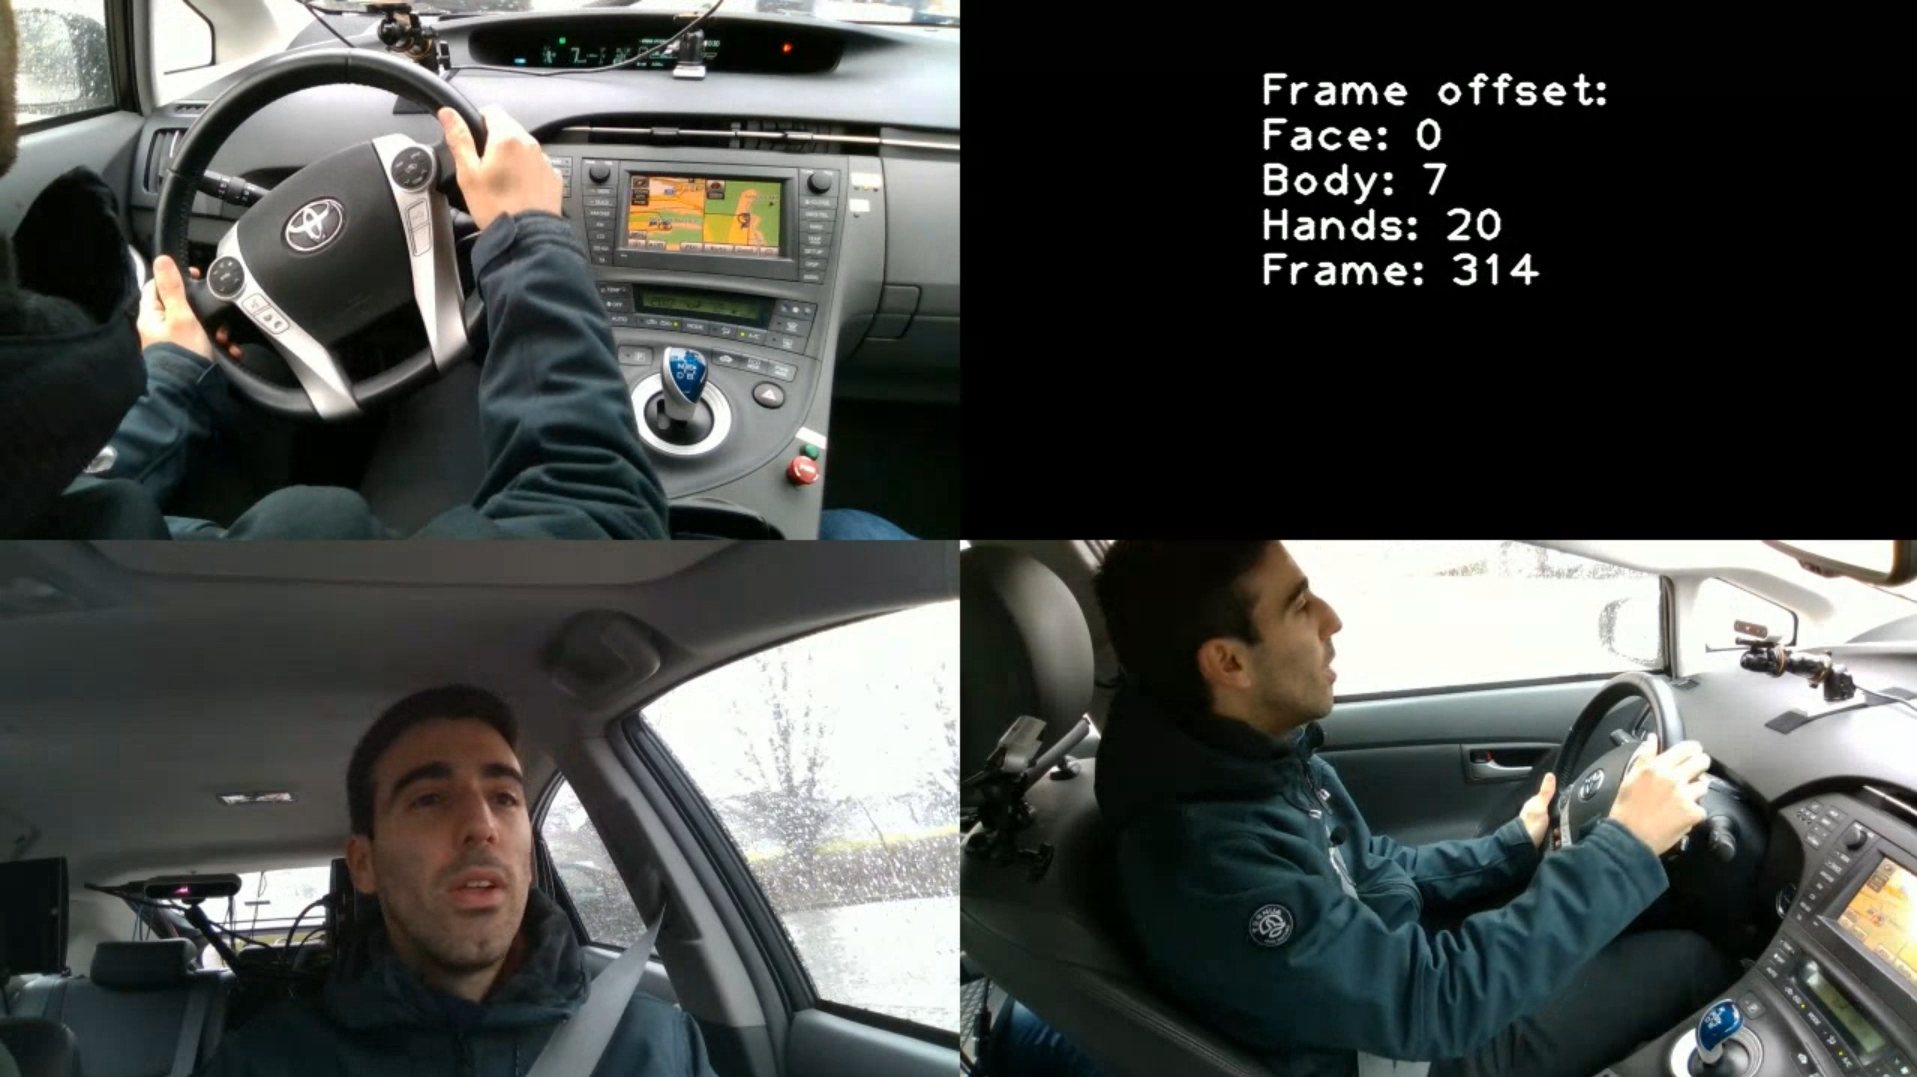
\includegraphics[width=0.5\linewidth]{figures/imagen muestra.png}
    \caption{Imágenes de cámaras disponibles en DMD(\cite{DMD})}
    \label{fig:muestra DMD}
\end{figure}

Para la metodología de este sistema solo se utilizan las 2 anotaciones en relación a la mirada del conductor con los nombres \textit{looking\_road} y \textit{not\_looking\_road}, estableciendo de manera binaria que el conductor se encuentra distraído si no tiene la mirada fija en la carretera. Ejemplos de las categorías se muestran en las Figuras \ref{fig:lr} y \ref{fig:nlr}  en las cuales se puede observar que precisamente el enfoque de categorización es en la mirada.

\begin{figure}[h!]
    \centering
    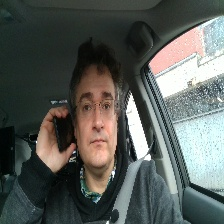
\includegraphics[width=0.3\linewidth]{figures/muestra lkr.jpg}
    \caption{Imagen de categoría \textit{looking\_road} (\cite{DMD})}
    \label{fig:lr}
\end{figure}

\begin{figure}[h!]
    \centering
    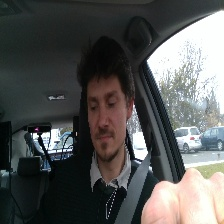
\includegraphics[width=0.3\linewidth]{figures/muestra nlkr.jpg}
    \caption{Imagen de categoría \textit{not\_looking\_road} (\cite{DMD})}
    \label{fig:nlr}
\end{figure}

\newpage %por ahora
El conjunto de datos cuenta con un total de 345,861 imagenes que pueden ser utilizadas para el entrenamiento de los modelos, de las cuales el 80\% (278,308) son de la categoría \textit{looking\_road} y un 20\% (67,553) de \textit{not\_looking\_road}. De manera inicial las clases presentan un desbalance de 4:1, por lo que es necesario implementar un balance de clases en el entrenamiento. 

\subsection{Modelos de aprendizaje profundo entrenados}
Se entrenaron múltiples arquitecturas de modelos de aprendizaje profundo con el objetivo de obtener un rango de resultados que ofreciera altos niveles de precisión con la mayor eficiencia computacional posible. Con este mismo propósito se empezaron con arquitecturas de redes neuronales convolucionales sencillas, siguiendo por arquitecturas de aprendizaje aprendizaje por transferencia, y finalmente un LSTM. LightGazeCNN es nuestra propia red neuronal convolucional de 4 capas ocultas. Cada capa cuenta con Batch Normalization, MaxPooling, y activación ReLU. Las capas ocultas tienen tamaño de 32, 64, 128 y 256. Para el aprendizaje por transferencia se entrenaron dos arquitecturas, MobileNetV3 y ResNet18. En la MobileNetV3 se descongelaron las últimas 2 capas. Para la ResNet18 se descongelaron las últimas 5 capas. Tras los primeros 3 entrenamientos, se reentrenaron con optimización de hiperparámetros la LightGazeCNN y ResNet18 que fueron las que mejores resultados entregaron inicialmente. Este procedimiento fue realizado con Optuna, y se optimizo el \textit{learning rate, batch size, weight decay, dropout}, optimizador, y en el caso de la ResNet18, cantidad de capas descongeladas. Finalizando con las CNN, se entreno una ultima vez la ResNet18 agregando preprocesamiento de imagen, aplicando escala de grises y CLAHE. Respecto al entrenamiento de la C-LSTM, se utilizó la ResNet18 como CNN y se agregó 1 capa de LSTM. Tras el primer entrenamiento, se realizó una optimización de hiperparámetros para la C-LSTM para los parámetros \textit{learning rate, batch size, weight decay, dropout}, optimizador y cantidad de capas y neuronas LSTM.

La Tabla \ref{tab:tabla arq} muestra los 8 experimentos realizados, incluyendo la cantidad de parámetros calculados en cada arquitectura, que funcionan como indicadores que consumo computacional

\begin{table}[h!]
    \centering
    \begin{tabular}{c|c}
          Arquitectura &  Num. de Parámetros \\
         \hline
         LightGazeCNN (CNN propia)  & 0.42M \\
         \hline 
         MobileNetV3  & 1.33M \\
         \hline
         ResNet18 & 8.39M \\
         \hline
         LightGazeCNN con optm. de hiperparametros & 0.42M \\
         \hline
         ResNet18 con optm. de hiperparametros & 10.49M \\
         \hline
         ResNet18 con optm. de hiperparametros + Grayscale \& CLAHE & 10.49M \\
         \hline
         C-LSTM & 10.88M \\
         \hline
         C-LSTM con optm. de hiperparametros & 10.88M \\
         \hline
    \end{tabular}
    \caption{Experimentos de entrenamiento de arquitecturas}
    \label{tab:tabla arq}
\end{table}

\subsection{Sistema de detección de distracción en tiempo real}
Con las redes neuronales convolucionales entrenadas, se aplicaron a un algoritmo en tiempo real que detecta distracción a través de las imágenes capturadas por la cámara del equipo. Buscando detección más robsuta y menos persistente, en el alogritmo de tiempor real se agregaron condiciones de detección, no solo tomando en cuenta la predicción del modelo de aprendizaje profundo frame por frame. Se aplico una ventana de 10 frames con la cuál se usa la moda de la predicción para indicar al conductor si esta distraido o no. Como ultimo filtro de detección se utiliza la norma establecida por la NHTSA que indica que un conductor no debe de estar distraido por más de dos segundos (\cite{NHTSA}). De esta manera, la alarma de distracción se activa solamente si la moda de la predicción de los últimos 10 frames es \textit{not\_looking\_road} durante 2 segundos. 

En la experimentación se realizaron pruebas de este codigo en una laptop para simular condiciones de poder computacional óptimas. La especificaciones de la computadora son: 

\begin{itemize}
    \item Procesador: 11th Gen Intel(R) Core(TM) i5-11400H @ 2.70GHz (2.69 GHz).
    \item RAM: 16GB
    \item Tarjeta gráfica: NVIDIA GeForce RTX 3050 Ti Laptop GPU (4 GB)
Intel(R) UHD Graphics (128 MB).
    \end{itemize}
    
También ese realizaron pruebas en una Rapberry Pi 5B, con el objetivo de generar comparativas entre la velocidad del algoritmo en distintas condiciones. Las especificaciones de la Raspberry Pi 5B son:

\begin{itemize}
    \item Procesador: Arm Cortex-A76 de cuatro núcleos y 64 bits a 2,4 GHz
    \item RAM: 16GB
    \item Tarjeta gráfica: VideoCore VII
    \end{itemize}
\section{Implementación en tiempo real}
\subsection{Equipo \textit{Plug-and-play}}
\subsection{Modularización de algoritmo y cambio de lenguaje Python a C++}
